Notre projet est basé sur l'architecture logicielle MVC (Modèle-Vue-Contrôleur) qui permet de séparer la logique métier de la présentation.
Nous avons ainsi identifié 4 modules principaux(voir figure \ref{fig:architecture}):
\begin{figure}[H]
	\centering
	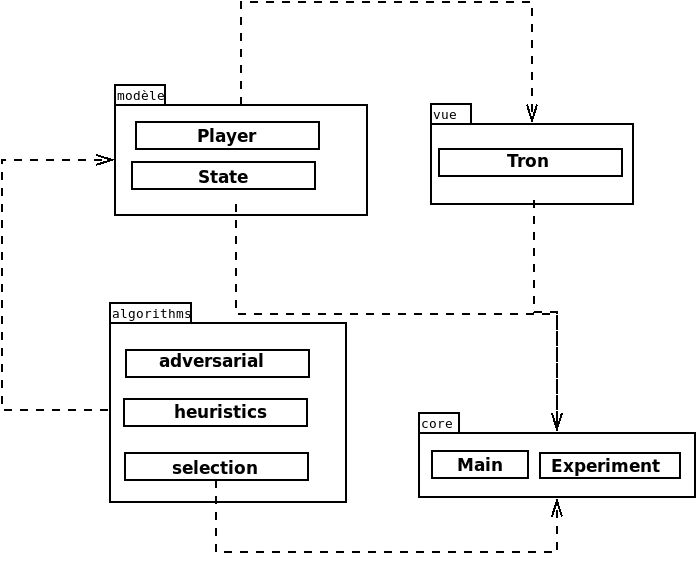
\includegraphics[scale=0.4]{diagrames/architecture}
	\caption{Architecture du projet}
	\label{fig:architecture}
\end{figure}

\begin{itemize}
	\item \textbf{Modèle} : Il contient les classes qui représentent les différents éléments du jeu comme les joueurs, la grille de jeu, etc. Il gère également les règles du jeu et les interactions entre les différents éléments.
	\item \textbf{Vue} : Il est responsable de l'affichage graphique du jeu et des interactions utilisateur. Il est constitué d'une interface utilisateur (UI) qui permet à l'utilisateur de jouer et de visualiser les différentes informations du jeu.
	\item \textbf{Core} : Contient l'ensemble des classes executables qui permettent de lancer le jeu.
	\item \textbf{algorithms}: Il contient l'ensemble des algorithmes de recherche adversarial, des techniques de selection et des heuristiques.
\end{itemize}
En somme, l'architecture MVC nous permet de séparer les différentes responsabilités de notre application, ce qui facilite la maintenance et l'évolution de notre code.
\subsection{Modules et Classes}
\subsubsection{Modèle}
Le modèle de notre application repose sur  plusieurs classes interdépendantes(voir figure \ref{fig:modele}) pour gérer l'état du jeu,
le plateau de jeu, les joueurs, leur position et leurs mouvements.
\begin{figure}[ht!]
	\centering
	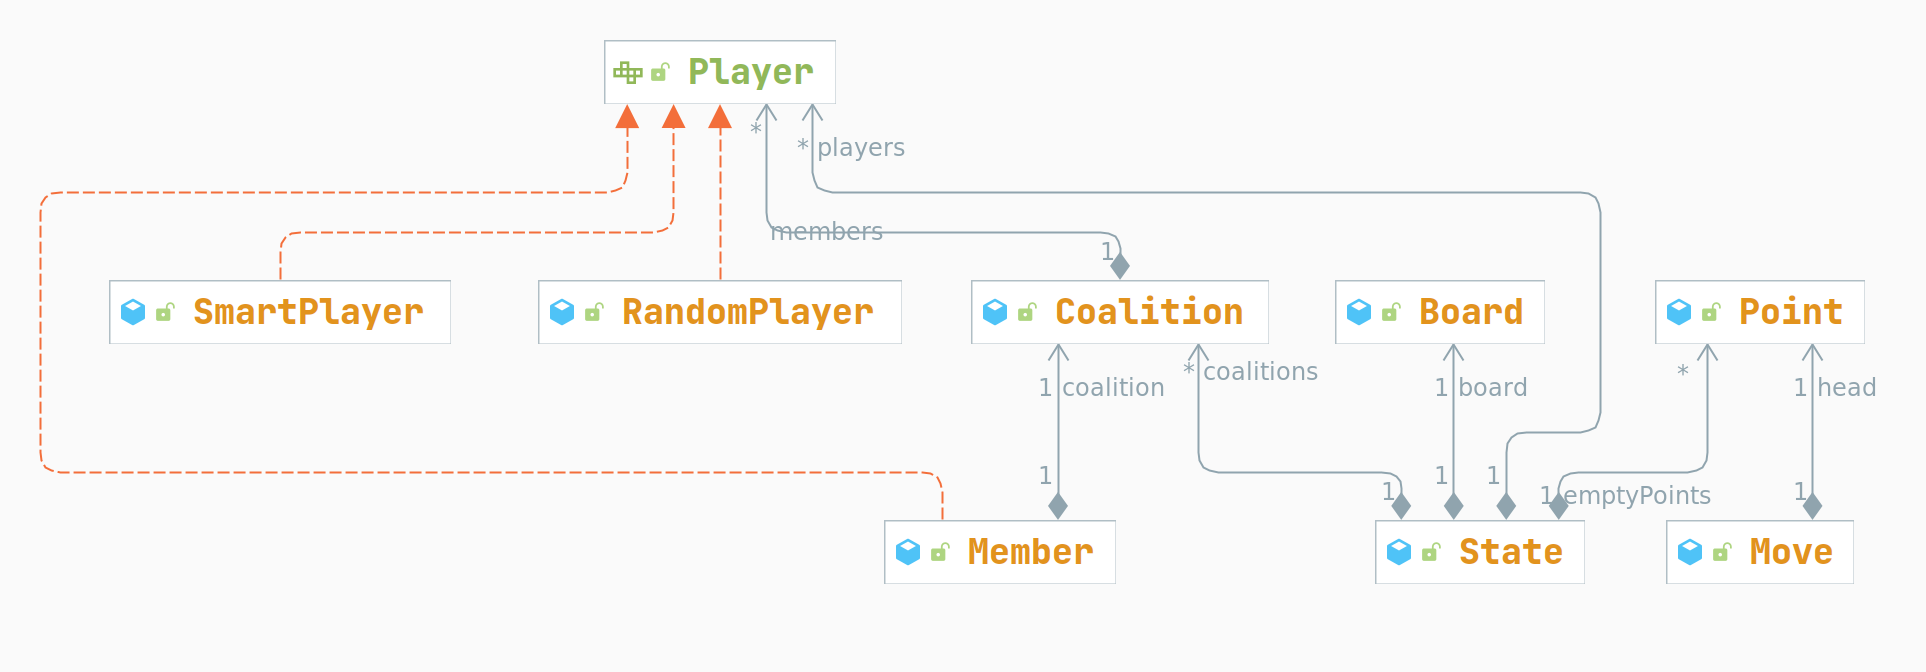
\includegraphics[scale=0.25]{diagrames/model}
	\caption{Diagramme de classe du modèle}
	\label{fig:modele}
\end{figure}\\


\tocless\paragraph{Move}
La classe Move est une classe importante de notre modèle qui représente le mouvement effectué par un joueur. Elle contient les 
informations nécessaires pour décrire un mouvement, à savoir la position final du joueur(dans notre cas la tête du joueur), la direction du mouvement et la longueur du mouvement qui a été effectué dans la même direction.
\begin{figure}[ht!]
	\centering
	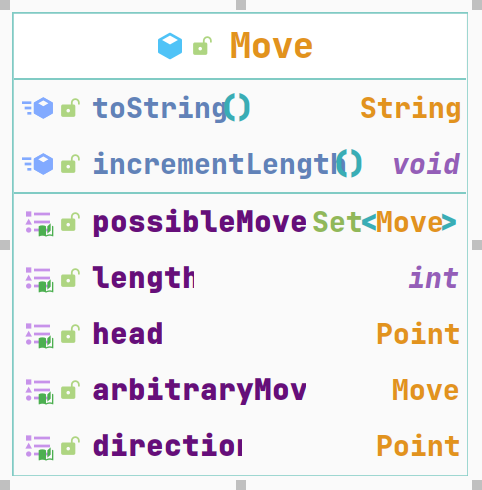
\includegraphics[scale=0.4]{diagrames/Move}
	\caption{Diagramme de classe de la classe Move}
	\label{fig:move}
\end{figure}
Grâce aux méthodes de la \classname{Move}(voir figure~\ref{fig:move}), on peut effectuer la validation d'un mouvement, obtenir la position final d'un mouvement, obtenir la direction d'un mouvement, obtenir la longueur d'un mouvement, etc.\\

Le choix de stocker la longueur d'un mouvement dans la classe \classname{Move}  découle du besoin de stocker les mouvements des joueurs dans une liste. 
En effet en considérant les mouvements effectués par le joueur rouge dans la figure~\ref{fig:heuristique},  si on stockait 
chaque position à un temps donné, on aurait eu besoin de stocker 20 éléments pour reconstituer le chemin du joueur rouge. Cependant, en utilisant notre implémentation, nous n'avons 
besoin de stocker que 9 mouvements, ce qui permet d'optimiser l'utilisation de la mémoire de notre application.\\

\tocless\paragraph{State}
La classe \classname{State} représente l'état du jeu à un instant donné. Elle contient les informations nécessaires pour décrire l'état du jeu(voir figure~\ref{fig:state}).
\begin{figure}[ht!]
	\centering
	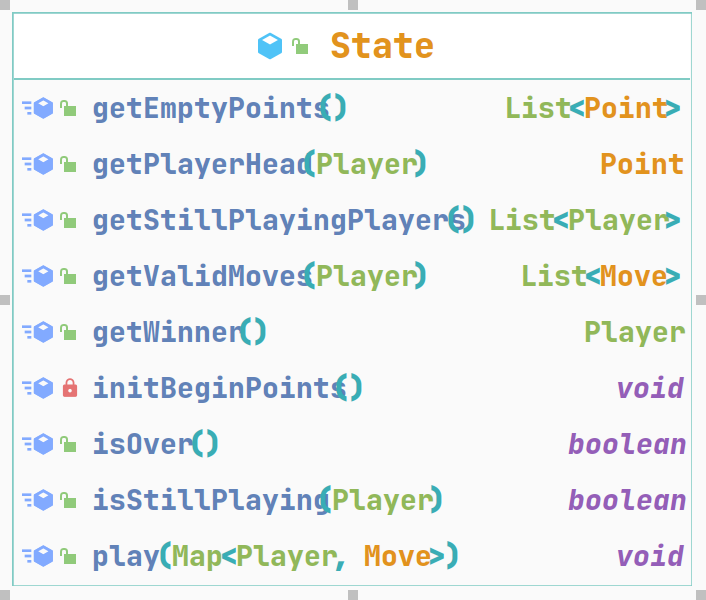
\includegraphics[scale=0.4]{diagrames/State}
	\caption{Diagramme de classe de la classe State}
	\label{fig:state}
\end{figure}\\

À travers cette classe, nous fournissons un objet permettant non seulement de pouvoir l'utiliser dans les algorithmes de recherche adversarial, mais aussi de pouvoir l'utiliser dans l'interface graphique pour afficher l'état du jeu.\\

L'une des principales méthodes de cette classe est la méthode \methodname{initBeginPoints} qui permet d'initialiser les positions initiales des joueurs.
Cette méthode est appelée dans le constructeur de la classe \classname{State} et permet de définir les positions initiales des joueurs. Pour un souci d'équitabilité, 
nous avons décidé de placer les joueurs de manière equidisante de centre du plateau de jeu. C'est à dire:
\begin{multline}
	\forall i ~\in ~$[0, nbJoueurs[$\\
	pos_x(i) = \frac{width}{2} + \frac{width}{2} \times \frac{2\pi i}{nbJoueurs}\\
	pos_y(i) = \frac{height}{2} + \frac{height}{2} \times \frac{2\pi i}{nbJoueurs}\\
\end{multline}
où $width$ et $height$ sont les dimensions du plateau de jeu et $nbJoueurs$ est le nombre de joueurs.\\

\subsubsection{Vue}
vue de l'application comporte des classes spécialement conçues pour faciliter l'interaction avec l'interface graphique 
utilisateur et pour offrir une représentation visuelle détaillée du déroulement des algorithmes et des parties. Elle permet à l'utilisateur de 
suivre les différentes étapes de l'exécution des algorithmes, de visualiser les mouvements des joueurs et d'observer le plateau de jeu de manière plus détaillée. 
En conséquence, la vue améliore significativement la compréhension et l'expérience de l'utilisateur lors de l'utilisation de l'application.

\tocless\paragraph{Les popups}
Les popups sont des éléments de l'interface graphique utilisateur qui sont utilisés pour fournir des informations supplémentaires à l'utilisateur ou 
pour les inviter à effectuer une action. Dans notre application, nous les avons utilisés pour afficher les informations relatives à la partie en cours tel que 
la fin de la partie, le gagnant, le nombre de coups joués(voir figure~\ref{fig:popupendgame}), etc.\\

\begin{figure}[H]
	\centering
	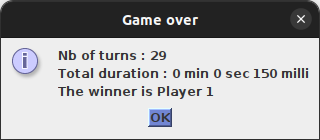
\includegraphics[scale=0.4]{Images/finjeu}
	\caption{Popup de fin de partie}
	\label{fig:popupendgame}
\end{figure}

En outre,  nous avons utilisé des fenêtres contextuelles pour permettre à l'utilisateur d'instancier les différentes IA qui s'affronteront sur le plateau et voir le récapitulatif global(voir figure~\ref{fig:fenetrecontextuelle}).
\begin{figure}[H]
	\centering
	\includegraphics[scale=0.4]{Images/récapitulatif}
	\caption{Fenêtre contextuelle}
	\label{fig:fenetrecontextuelle}
\end{figure}
Cette fonction est particulièrement utile car elle permet à l'utilisateur de sélectionner et de modifier les paramètres des différentes IA, tels que leur profondeur 
ou leur fonction heuristique. En fournissant ces fenêtres contextuelles, nous sommes en mesure d'améliorer l'expérience de l'utilisateur et de rendre l'application plus conviviale et intuitive.

\tocless\paragraph{La fenêtre de jeu}
La fenêtre principale du jeu sert d'interface principale pour afficher l'état actuel du jeu. Elle se compose de trois parties principales(voir figure~\ref{fig:fenetrejeu})

\begin{figure}[H]
	\centering
	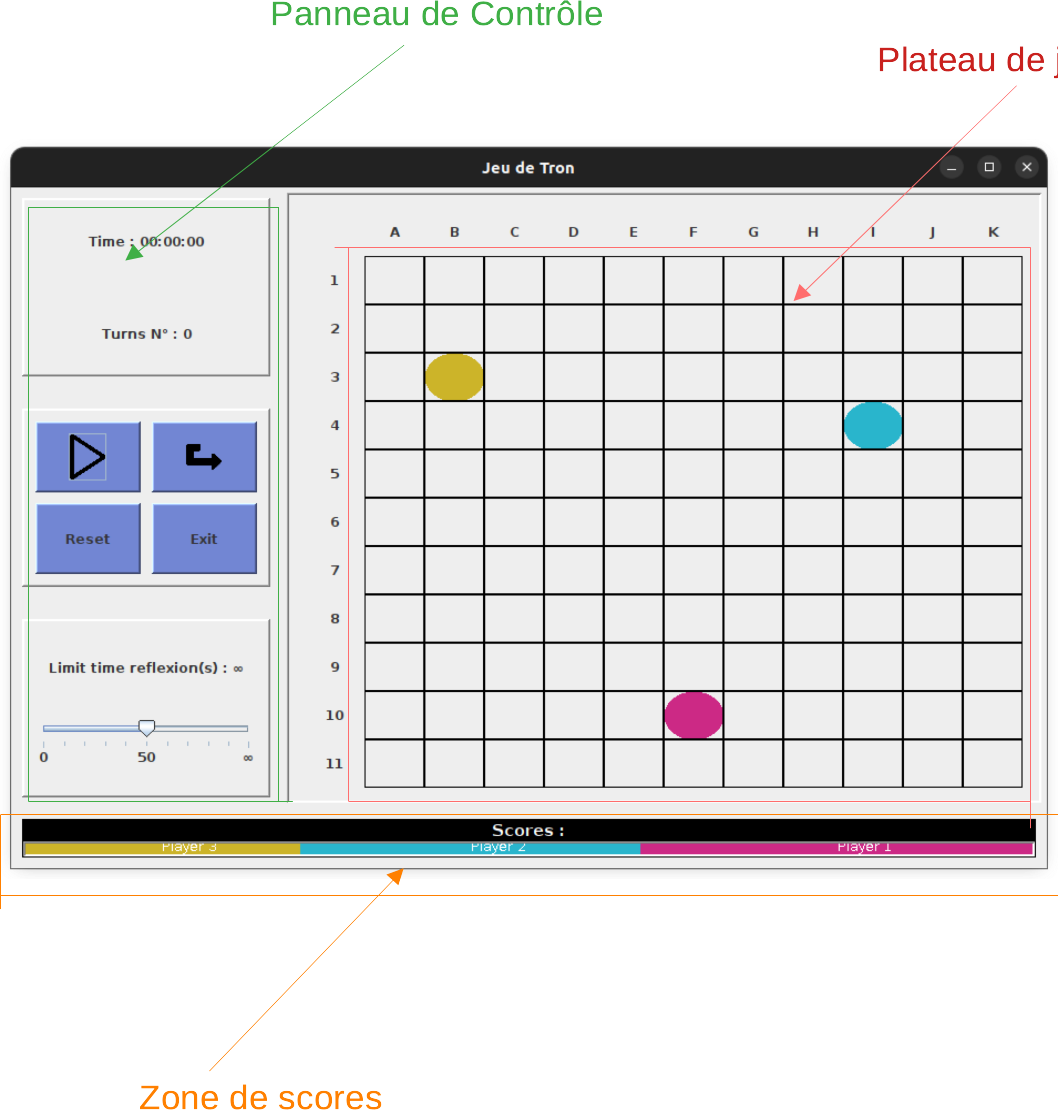
\includegraphics[scale=0.35]{Images/fenetrejeu}
	\caption{Fenêtre principale du jeu}
	\label{fig:fenetrejeu}
\end{figure}

Le plateau de jeu est une grille qui représente le terrain de jeu et affiche la position actuelle des joueurs. La zone de score fournit une représentation graphique de la zone 
occupée par chaque joueur sous la forme d'un graphique à barres. Le panneau de contrôle contient divers boutons et commandes, notamment les boutons de démarrage, de réinitialisation et 
d'étape suivante, ainsi que des informations sur le nombre de tours, la durée du jeu et un curseur permettant d'ajuster le temps de réflexion d'un algorithme.\\

\subsubsection{Algorithmes}
Le package \packagename{algorithms}  contient tous les algorithmes spécifiques que nous avons mis en œuvre pour le jeu(voir figure~\ref{fig:algorithms}).
\begin{figure}[H]
	\centering
	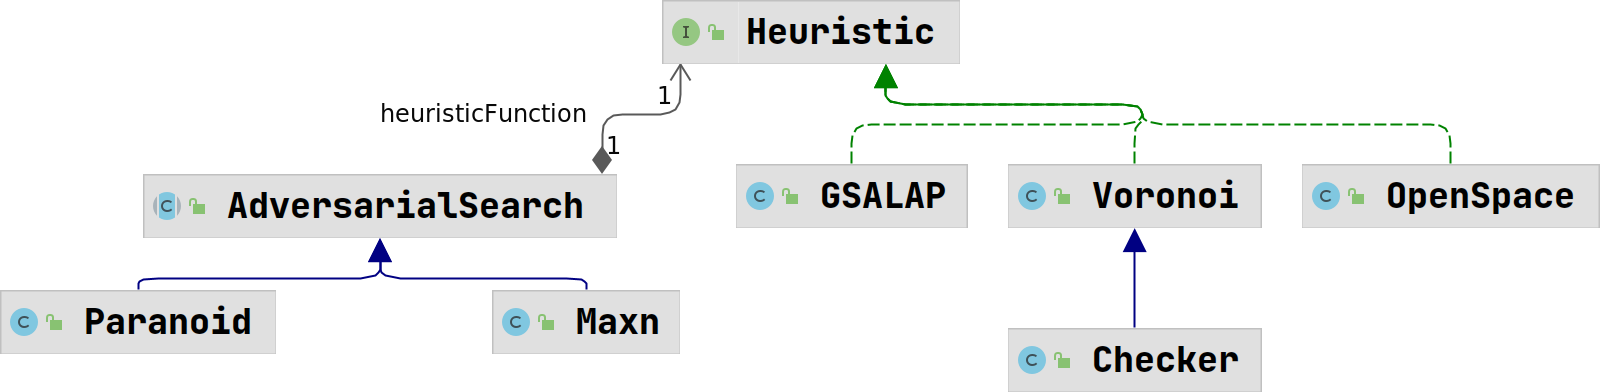
\includegraphics[scale=0.3]{diagrames/algorithms}
	\caption{Diagramme de classe du package algorithms}
	\label{fig:algorithms}
\end{figure}

Ces algorithmes sont classés en deux catégories :
\begin{itemize}
	\item les algorithmes de recherche adversarial
	\item les heuristiques(voir section~\ref{sec:analyse})\footnote{Les heuristiques sont utilisées pour évaluer les états du jeu et les comparer entre eux. Elles sont utilisées par les algorithmes de recherche adversarial pour
	déterminer le meilleur mouvement à effectuer.}
\end{itemize}

\subsection{Les fonctionnalités}
L'application offre diverses fonctionnalités qui permettent à l'utilisateur d'interagir avec le jeu, les algorithmes et l'interface. 
Les principales fonctionnalités sont les suivantes :
\begin{itemize}
	\item \textbf{Configuration de la partie} : : l'utilisateur peut configurer le jeu en définissant la taille du plateau, le nombre de joueurs et les algorithmes à utiliser.
	\item \textbf{Coloration d'un joueur} : Une couleur est attribuée à chaque joueur(couleur aléatoire variant d'une partie à l'autre) et est utilisée pour représenter le joueur sur le plateau de jeu.
	\item \textbf{Contrôle du jeu} : l'utilisateur peut démarrer, mettre en pause, reprendre et réinitialiser le jeu. L'utilisateur peut également avancer dans le jeu un coup à la fois.
	\item \textbf{Configuration des joueurs} : On peut configurer le temps de réflexion, la profondeur maximale de la recherche et les poids des heuristiques utilisées dans les algorithmes.
	\item \textbf{Sélection des algorithmes} : l'utilisateur peut choisir les algorithmes(recherche adversarial et heuristique) à utiliser pour chaque joueur.
	\item \textbf{Visualisation} : l'utilisateur peut visualiser les mouvements des joueurs et les étapes de l'exécution des algorithmes.
	\item \textbf{Statistiques du jeu} : l'application affiche diverses statistiques pendant et après le jeu, telles que le nombre de coups, la durée du jeu et les scores de chaque joueur.
	\item \textbf{Personnalisation de l'interface utilisateur} : l'utilisateur peut personnaliser l'interface utilisateur notamment en redimensionnant la fenêtre principale du jeu.
\end{itemize}





